\chapter{Forecasting the daily electricity consumption}
\label{cha:Forecasting the daily electricity consumption}
In this chapter the different forecasting techniques to perform a 24 hour prediction for an individual household are discussed. One daily prediction has a data granularity of an half hour, which means that $ 48 $ data points have to be estimated for each prediction. \\\textbf{update --> discussing data}
First pre-processing is done in Section \ref{s:Pre-processing} and the time series used are discussed. Afterwards the baseline models are looked into in Section \ref{s:Baseline models}. These models are characterised by a low calculation load during training and they therefore serve as an easy to obtain result where a more complex model can be compared with. Next, more complex models based on a neural network philosophy are discussed in Section \ref{s:Neural network models}. ``Long Short-Term Memory'' and ``Gated Recurrent Unit'' are most suitable to process time series and therefore serve as the core model which is analysed with different design choices. Finally, a parameter search is conducted. Here, an analysis is made of the sensitivity of the choice of different parameters is made.\\
 
\section{Pre-processing}\label{s:Pre-processing}
The data that is available is summarized by Table \ref{tab:available_data}. 

\subsection{Data}
In order to reduce the calculation load to do the parameter search in Section \ref{s: Parameter search}, three series are selected from the \textit{consumption.csv} that is listed in Table \ref{tab:availablef_data}. The series are chosen based on the least missing values of the historic electrical consumption serie and the absence of a big shift. Figure \ref{fig:three_series} shows the three figures and Table \ref{tab:three_series} summarizes their characteristics.\\

\begin{figure}[ht]
	\begin{subfigure}{0.32\textwidth}
		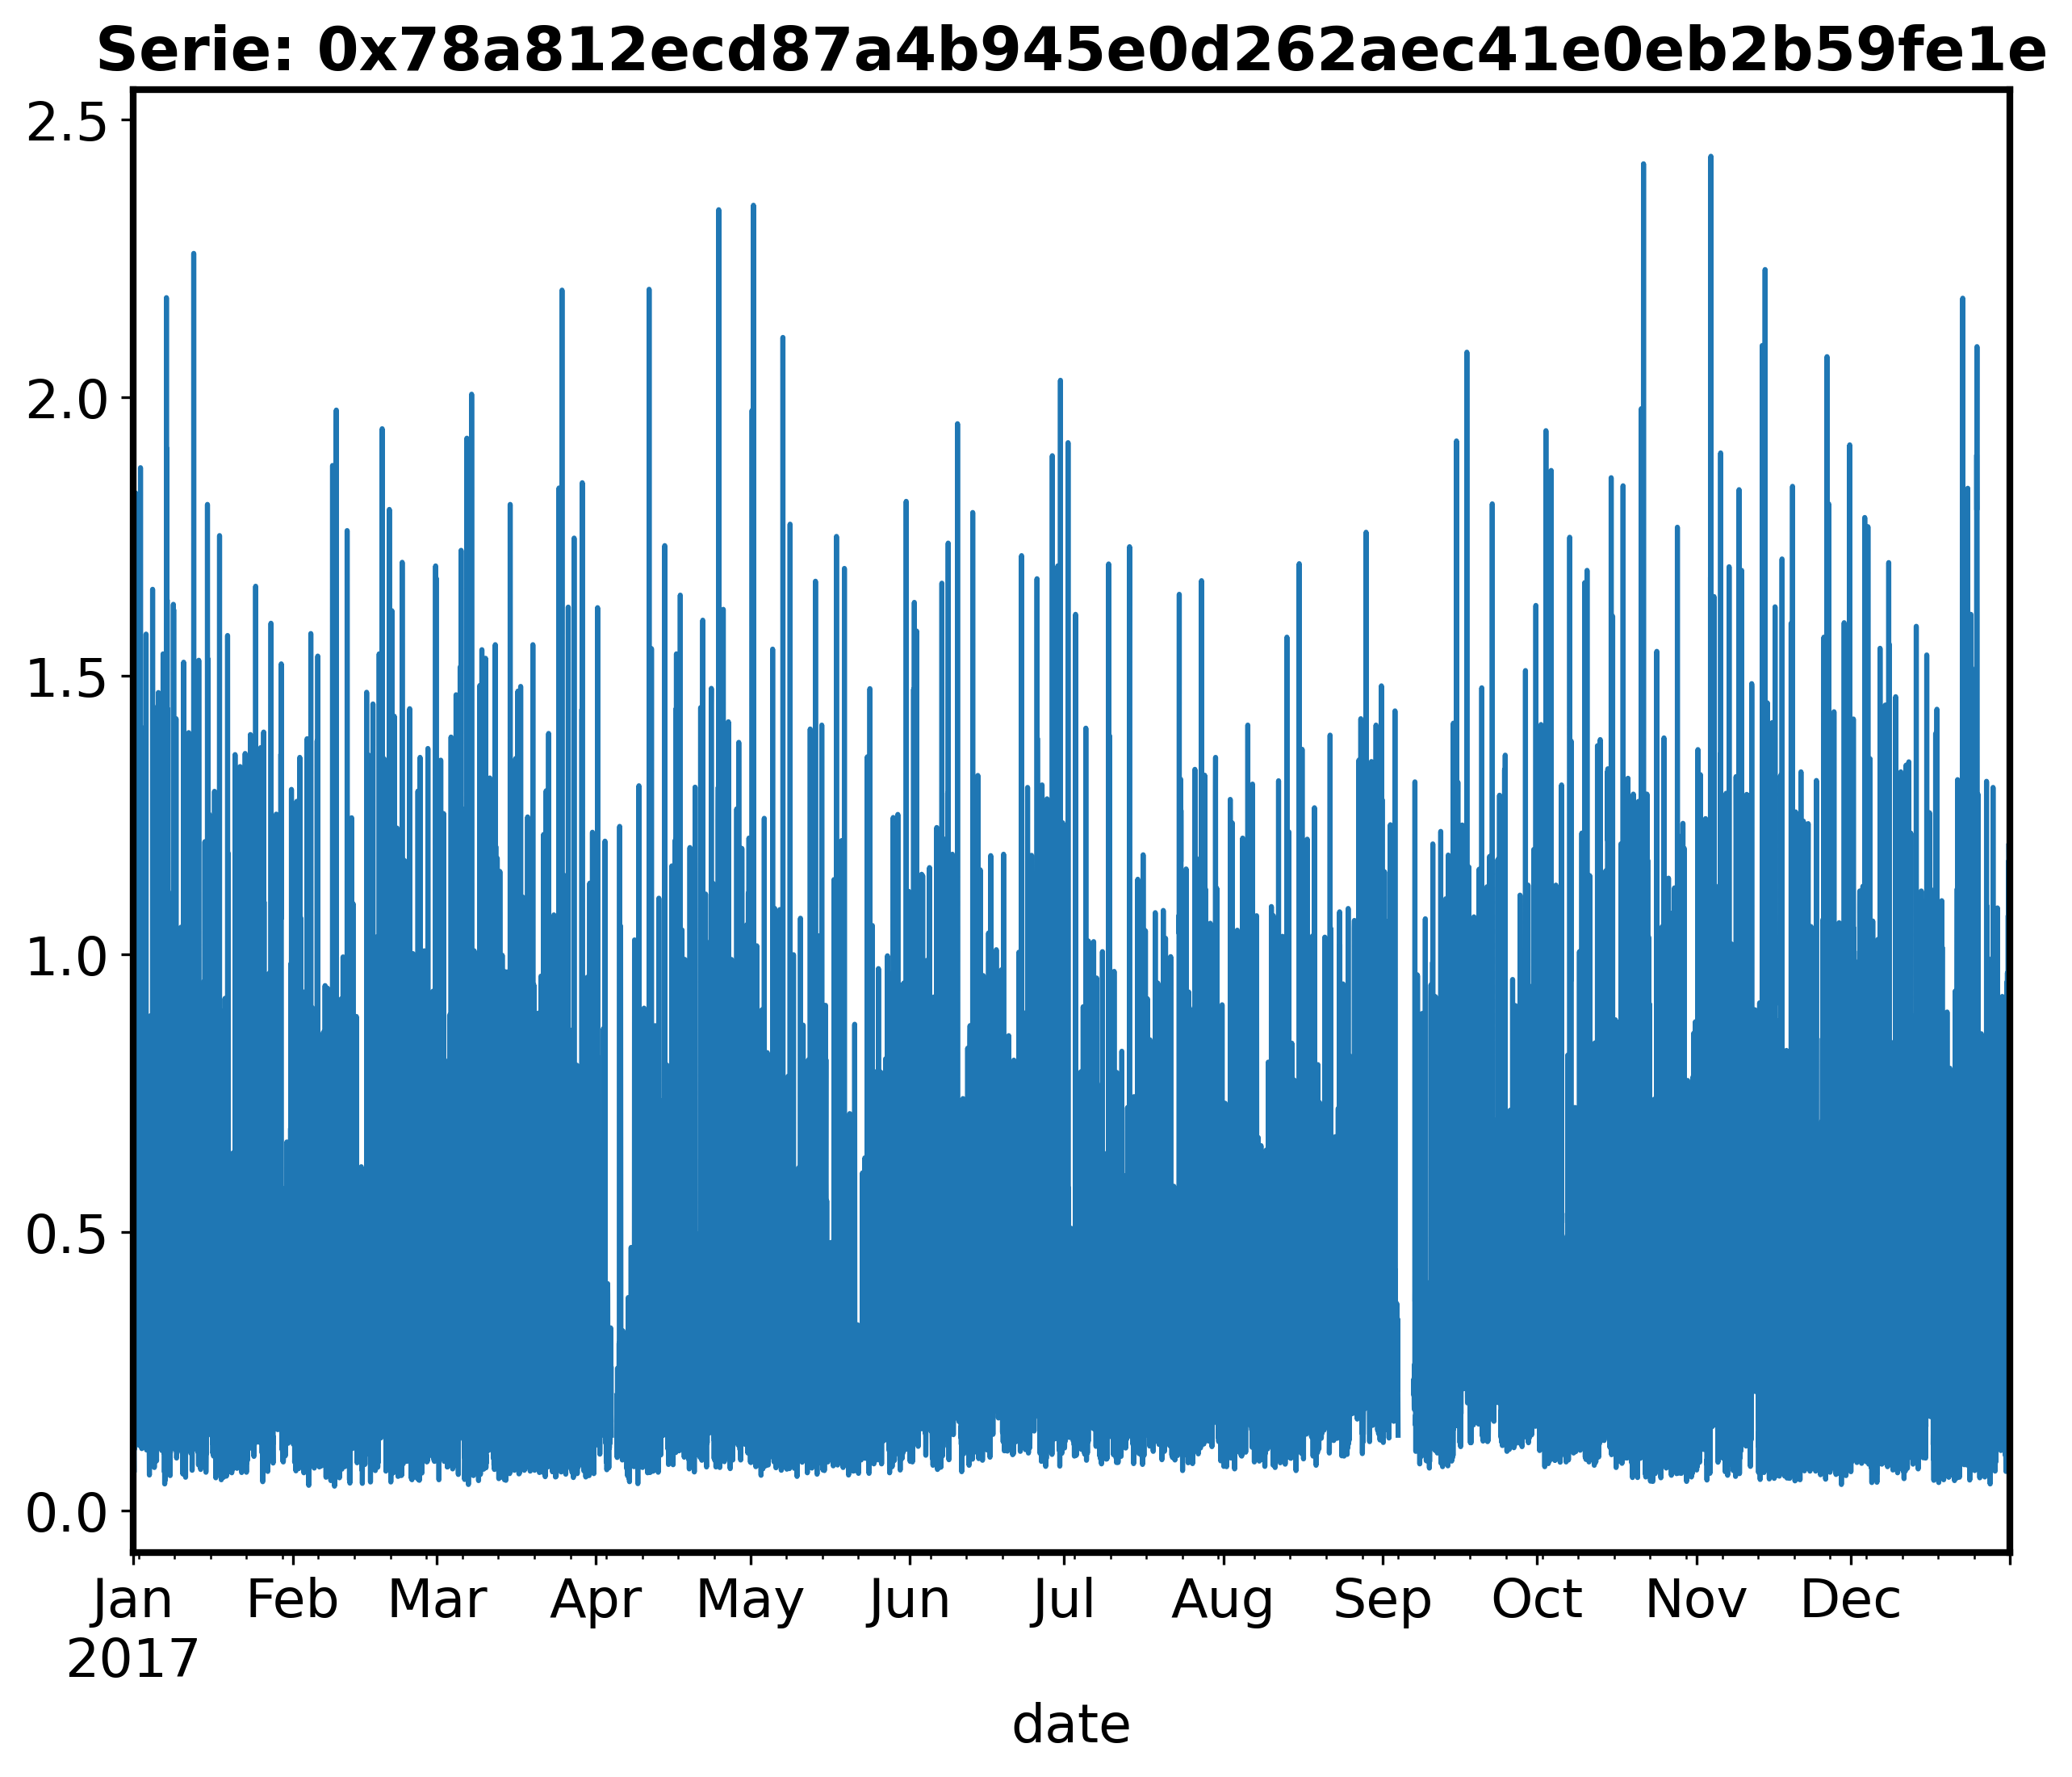
\includegraphics[width=1\linewidth]{Serie0x78a812ecd87a4b945e0d262aec41e0eb2b59fe1e.png}
		\caption{Serie $ 1 $}
	\end{subfigure}	 	
	\begin{subfigure}{0.32\textwidth}
		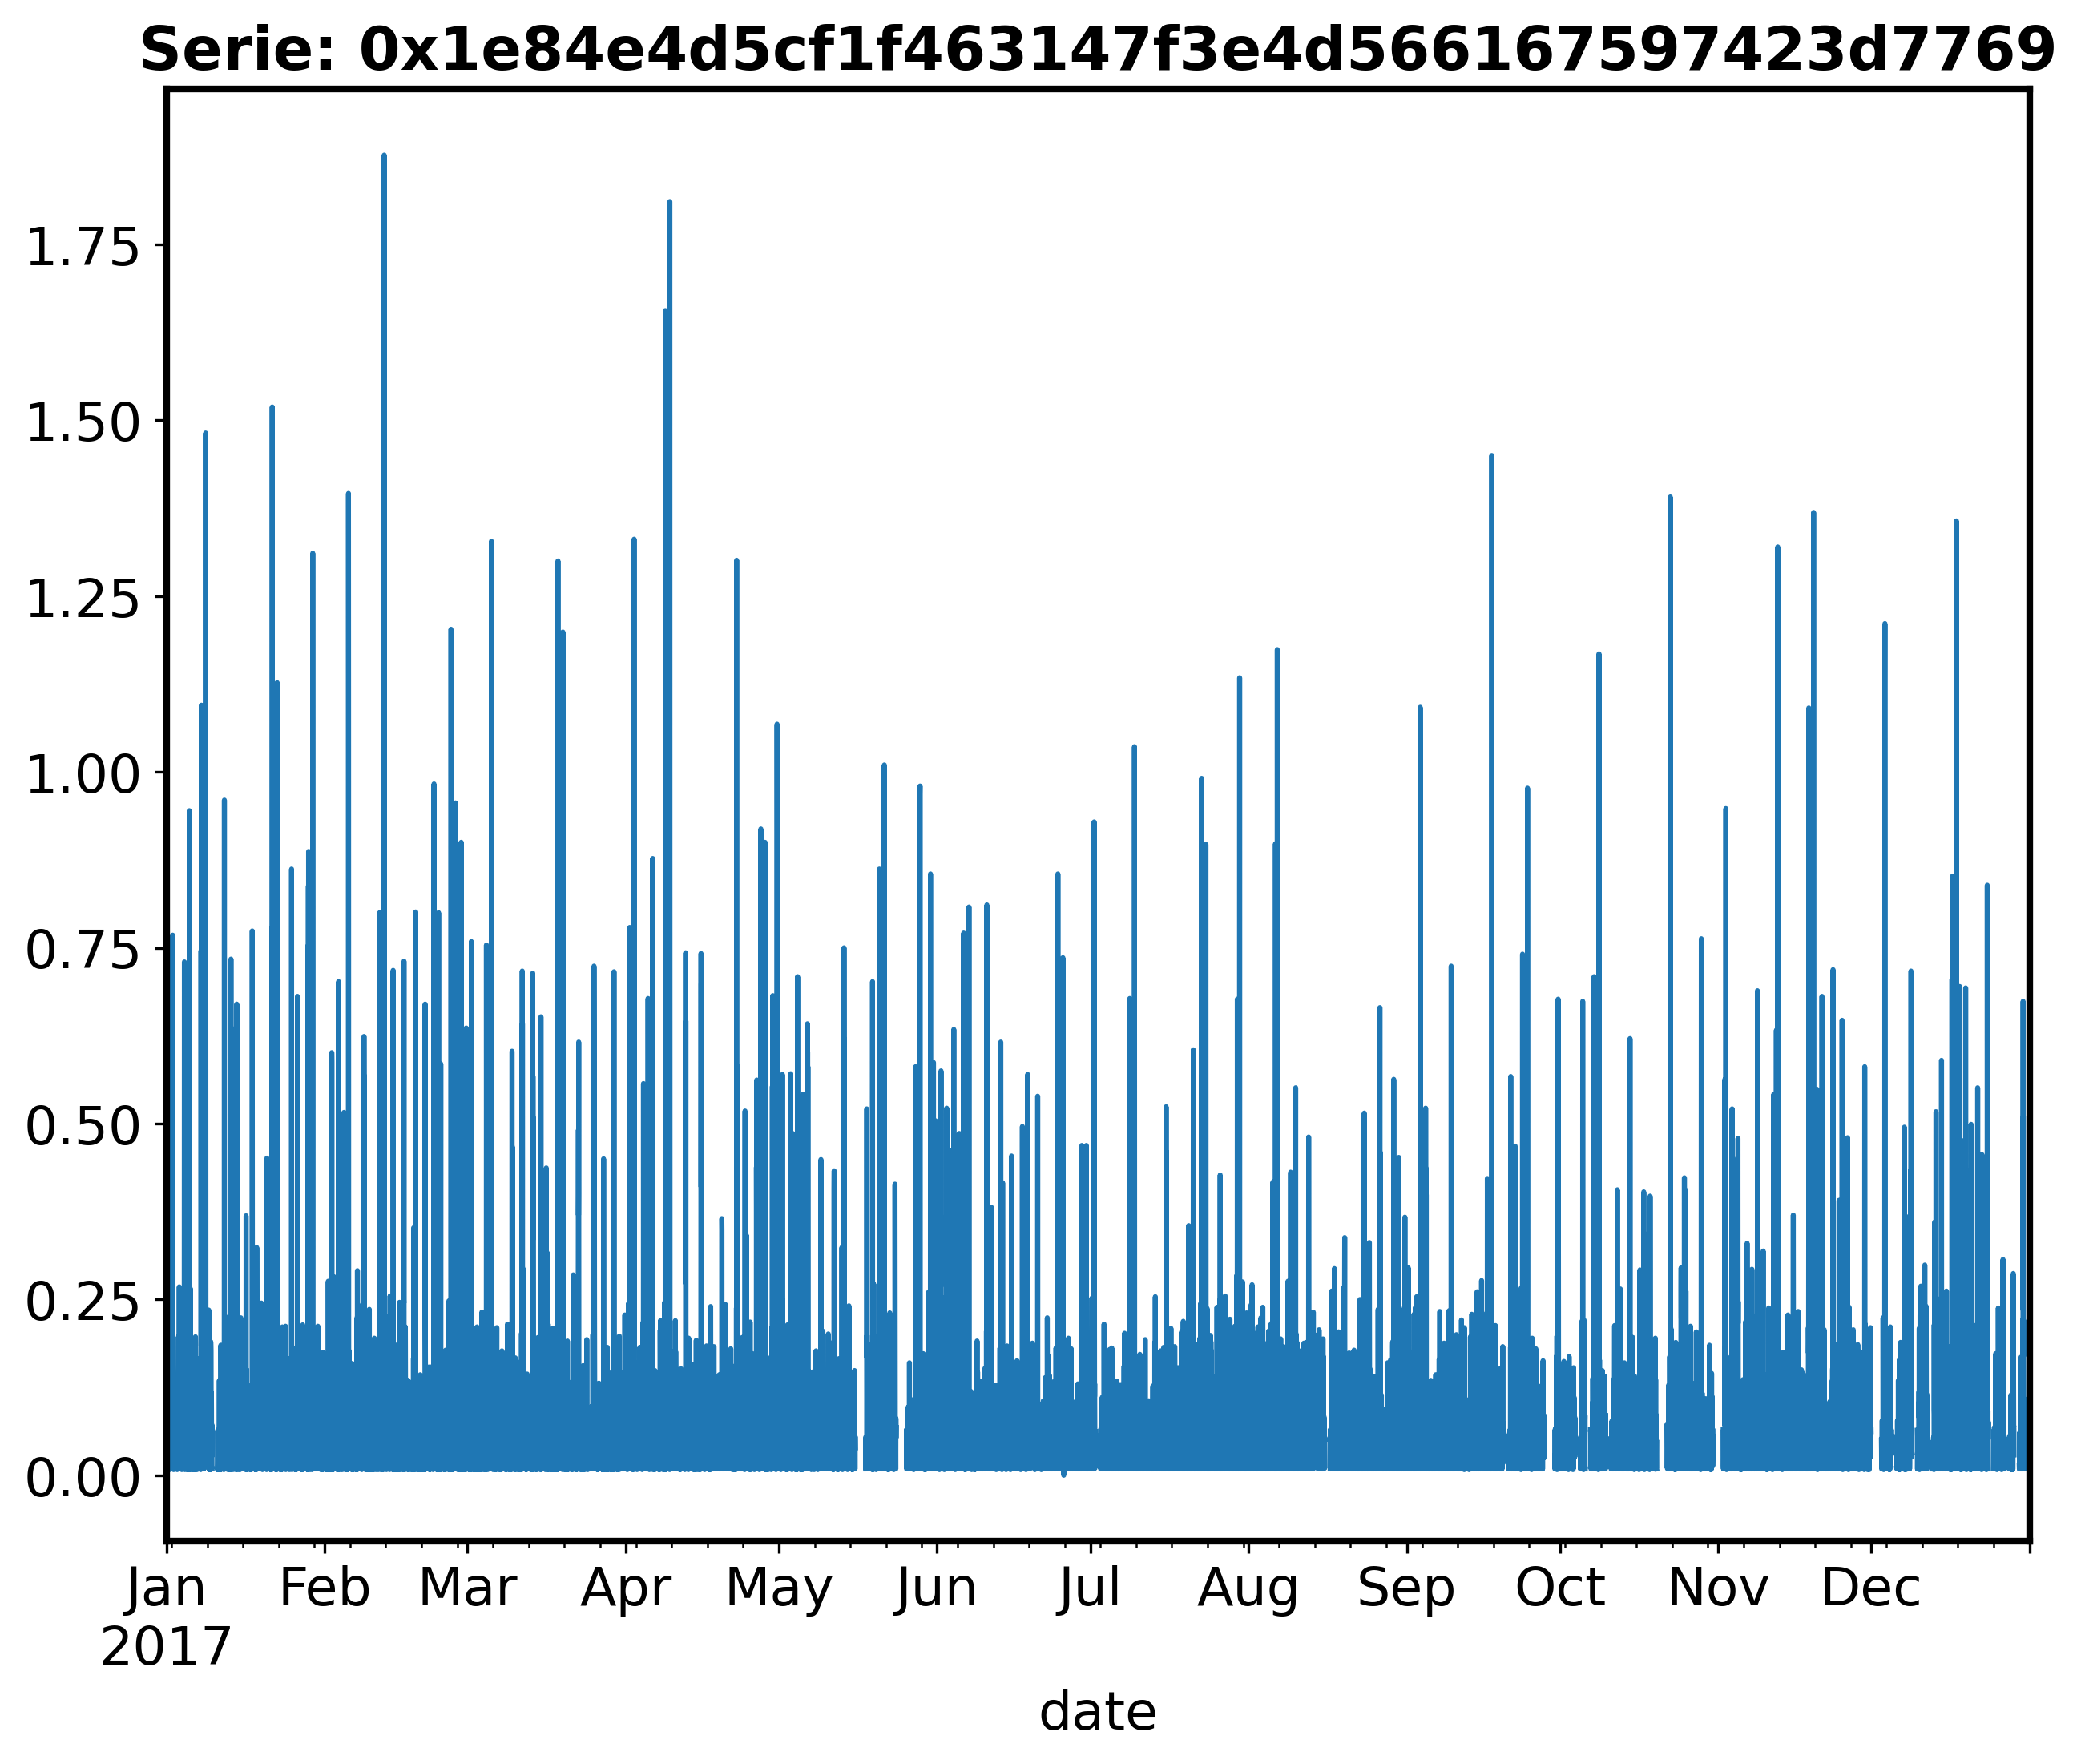
\includegraphics[width=1\linewidth]{Serie0x1e84e4d5cf1f463147f3e4d566167597423d7769.png}
		\caption{Serie $ 2 $}
	\end{subfigure}	
	\begin{subfigure}{0.32\textwidth}
		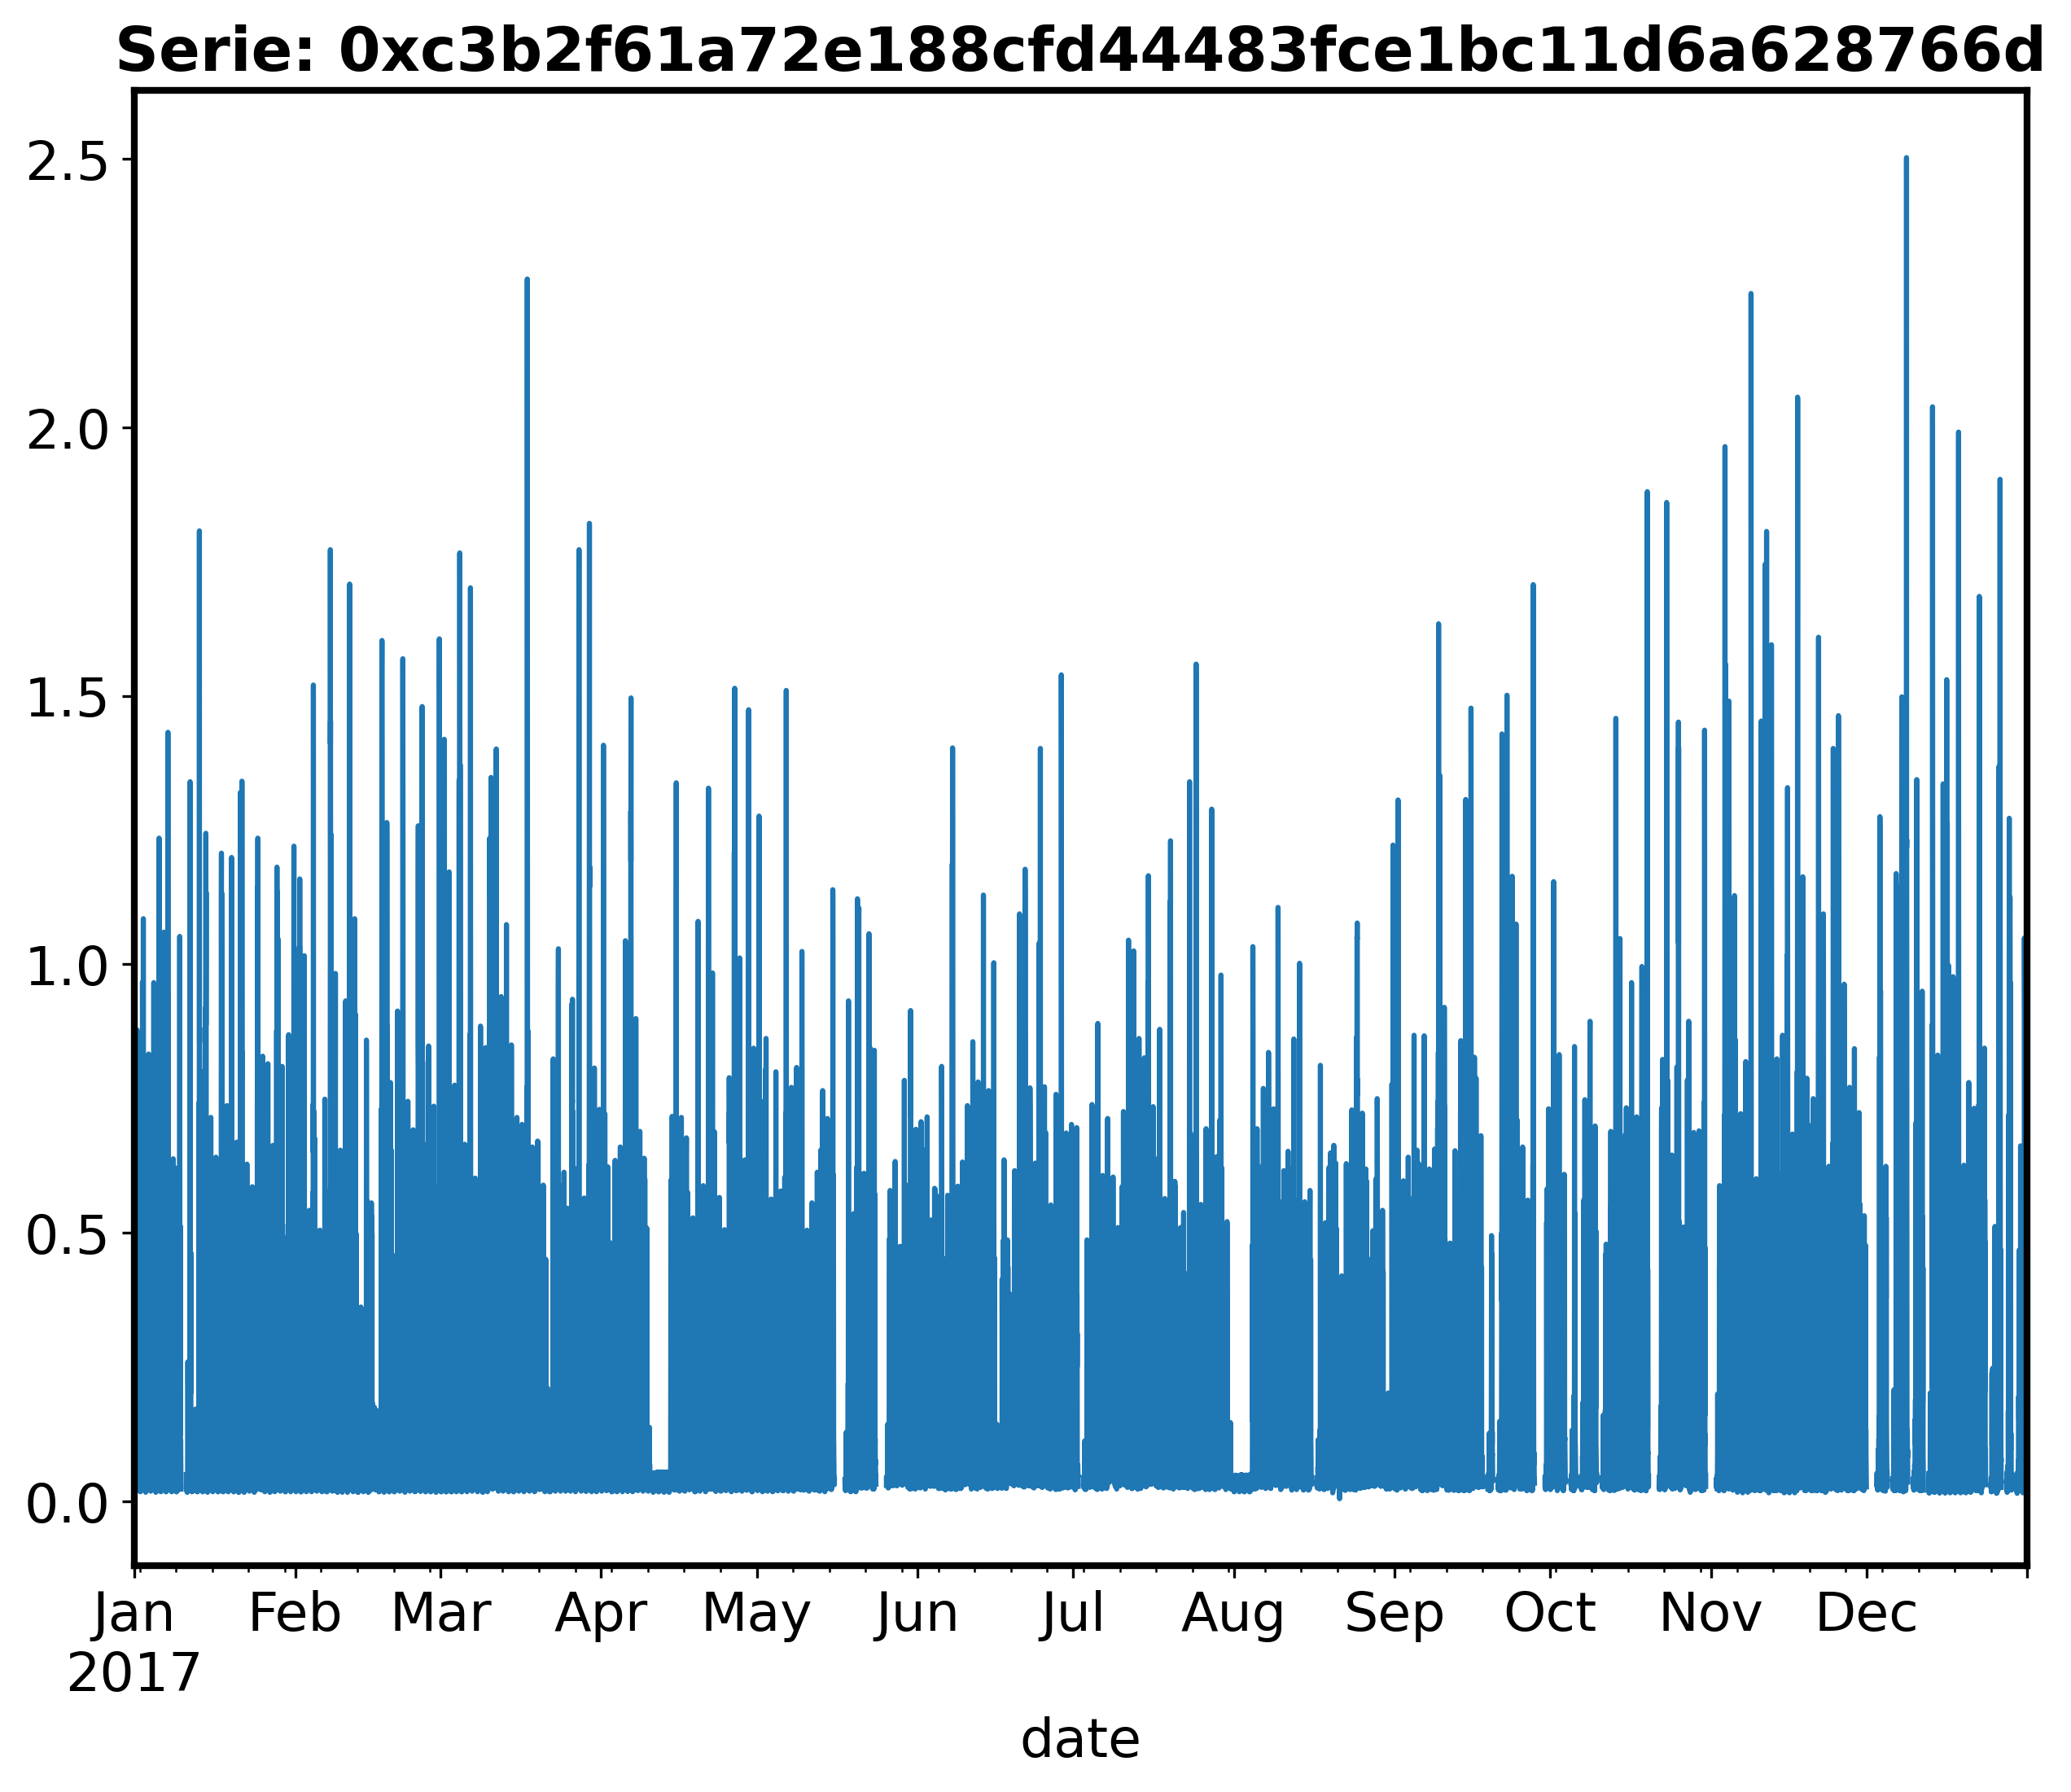
\includegraphics[width=1\linewidth]{Serie0xc3b2f61a72e188cfd44483fce1bc11d6a628766d.png}
		\caption{Serie $ 3 $}
	\end{subfigure}
	\caption{The consumption of $ 2017 $ for the three selected series. }
\end{figure}

\begin{table}
  \centering
  \begin{tabular}{@{}l|llr@{}} \toprule
  	\textbf{Characteristic}	& \textbf{Serie $ 1 $} & \textbf{Serie $ 2 $} & \textbf{Serie $ 3 $}\\\midrule
    Mean daily consumption [kWh]& $ 14.55 $&$ 3.17 $  & $ 6.58 $ \\
    Standard deviation daily consumption [kWh] &$ 3.21 $ & $ 0.99 $& $ 2.57 $ \\
    Median daily consumption [kWh] & $ 14.09 $ & $ 2.96 $& $ 5.88 $ \\
    Maximum daily consumption [kWh] & $ 30.08 $ & $ 6.60 $ &  $ 17.15 $   \\
    Minimum daily consumption [kWh]& $ 7.51 $ & $ 1.83 $ &  $ 1.50 $   \\
    Total missing days (consumption) & $ 4 $ &$ 25 $ & $ 26 $\\
    Days in validation set (November)&  $ 30 $ & $ 29 $  & $ 29 $ \\
    Days in Test set (December) & $ 31 $  $ 23 $  &    $ 31 $  & $ 23 $ \\
    Days in training set (Rest)&   $ 300 $  &  $ 288 $   &  $ 287 $\\
    Mean average temperature [$\degree C$]& $ 10.37 $  &  $ 10.61 $  & $ 10.22 $ \\
    Standard deviation average temperature [$\degree C$]& $ 5.09 $  & $ 5.20 $   & $ 5.01 $ \\
    Median average temperature [$\degree C$] &  $ 10.46 $ &  $ 10.61 $  & $ 10.35 $ \\
    Maximum average temperature [$\degree C$] & $ 23.99 $  & $ 24.51 $   & $ 22.95 $ \\ 
    Minimum average temperature [$\degree C$] & $ -1.07 $  &  $ -1.28 $  & $ -1.42 $ \\
    Missing average temperature days &  $ 0 $ & $ 0 $  & $ 0 $  \\ 
    Amount of holidays in $ 2017 $ & $ 8 $  &  $ 8 $  & $ 8 $ \\\bottomrule
  \end{tabular}
  \caption{summarizing characteristics about the selected series.}
  \label{tab:summ_data}
\end{table}

The three time series are divided in a training, validation and test set. As validation and test set are respectively the months November and December chosen. Because in this chapter the time series are not aggregated to a single signal as was the case in Section \ref{s:Analysis} the min-max normalization can be used. The missing values in the consumption are substituted by making use of following baseline models in order: ``previous week'' model, ``previous day'' model and the mean model. When a baseline can't make a forecast because the data is not available, a next baseline model is used. Similar, the missing values of the temperature are substituted by first looking at the temperature yesterday, then tomorrow and as last the mean temperature.\\

The simulations that are done in the chapter are performed on a virtual machine through the Microsoft Azure service.
Table \ref{tab:CPU} shows the different features of the hired machine. 
\begin{table}[hb]
	\centering
	\begin{tabular}{|p{2cm}|p{2cm}|p{2cm}|p{2cm}|}\hline
		\textbf{Name}	& \textbf{Logical cores} & \textbf{RAM (GB)} & \textbf{Storage (GB)}\\\hline
		F4s v2& $ 4 $&$ 8 $  & $ 32 $ \\\hline
	\end{tabular}
	\caption{Specifications of the virtual machine.}
	\label{tab:CPU}
\end{table}


\textbf{- Make a table that summarizes the environment to do simulations.(baseline and othe models) (can be put in the appendix)}
\section{Baseline models}\label{s:Baseline models}
\subsection{Models}
As earlier discussed, the baseline models are characterised by a low calculation load during training and therefore serve as a baseline to compare more complex models with. The different baseline models tried are listed as follows:
\begin{itemize}
	\item Model 1: ``closest day forecast''
	\item Model 2: ``1 day ago forecast''
	\item Model 3: ``7 days ago forecast''
	\item Model 4: ``Mean forecast''
	\item Model 5: ``MAPE forecast''
\end{itemize} 

For all the models listed here, the training set for the forecast of the next day are all the days before this day of the year $ 2017 $. These models can therefore be categorized as ``lazy learning models'' because they only do work when they are asked a query. In contrast, the models discussed in Section \ref{s:Neural network models} generalize the training data without knowing the actual query. They belong to the ``eager learning methods'' class. The 24 hour predictions made by the $ 5 $ models are done all at once. This is in contrast to the models described in Section \ref{s:Neural network models}, where the prediction is made sample per sample and where the predictions done for an earlier hour of the day are taken into account.\\

\textbf{Model 1: ``closest day forecast''}\\
This model looks for the most similar day in the training set based on following metrics to make a prediction:

\begin{itemize}
	\item Holiday
	\item Day of the week
\end{itemize}

 All the days in the training are categorized according to these metrics. Then it is looked in which category the desired day belongs i.e. which day of the week and if it is a holiday. Inside the selected category, an assessment of the difference in average temperature is made for all days with respect to the desired day. It is assumed that the average temperature of the desired day is already available, which is a very plausible assumption. Finally, the day with the closest euclidean distance in temperature is selected and the electrical consumption signal is copied to serve as the prediction of the desired day. It should be noted that there are only a maximum of $ 8 $ holidays as can be seen in Table \ref{tab:summ_data}. Therefore, when a holiday should be predicted all Sundays are also included in the training set because a Sunday behaves most similar to a holiday as can be seen in Figure \ref{fig:sim_weekdays}.\\
 
 \textbf{Model 2: ``1 day ago forecast''}\\
 This model simply looks at the consumption of the day before the desired day. The philosophy of the model is that the most recent consumption data serves as a a good predictor.
 
 \textbf{Model 3: ``7 days ago forecast''}\\
 This model looks at the most recent household consumption of the previous corresponding day of the week. It is expected that people have a reasonably fixed routine during the week and therefore it is likely that this routine will also be found back in the electrical consumption.\\
 
 \textbf{Model 4: ``Mean forecast''}\\
 In the mean forecast the different days are again categorized as was done in Model $ 1 $, but instead of selecting a single day out of the group of days, a mean day is calculated and used as prediction of the desired day. No extra Sundays are included to forecast a holiday.\\
 
 \textbf{Model 5: ``MAPE forecast'' }\\
 This model solves for each half hour of the desired day a small non-linear optimization problem displayed by (Eq. \ref{eq:model_mape}). This model served as baseline model in paper \cite{Kong2019}. 
 
 \begin{equation}\label{eq:model_mape}
 	objective = \sum_{i=1}^K \zeta_{pi}\abs{\frac{(\hat{y}-p_i)}{pi}}
 \end{equation}
 
 Again a group of days of size $ M $, corresponding the desired day is selected based on the metrics of weekday and if the desired day is a holiday. Also Sundays are added to the group of holidays for this model. Next, the consumption at time $ t $ is extracted out of this group of days, which gives a list of length $ M $ with historic consumption values. From these values an empirical probability mass function $ \zeta_{pi} $ is derived by making use of a histogram using ``Freedman-Diaconis rule'' to decide the bin size. Figure \ref{fig:histogram_mape} shows an example of such an histogram. The amount of discretized values $ p_i $ is equal to the $ K $ bins and taken as the midpoint of two bin edges. From the count in the histogram the probability mass function for each discretized value is found. $ \hat{y} $ is found by minimizing equation \ref{eq:model_mape}.\\
 
The metrics used to evaluate the predictions performance of the baseline models are $ RMSE $ (Eq. \ref{eq:RMSE}), $ NRMSE $ (Eq. \ref{eq:NRMSE}), $ MAE $ (Eq. \ref{eq:MAE}), $ MSE $ (Eq. \ref{eq:MSE}) and $ MAPE $ (Eq. \ref{eq:MAPE}).

\begin{equation}\label{eq:MSE}
	MSE = \frac{\sum_{t=1}^{N}(\hat{y}_t-y_t)^2}{N}
\end{equation}

\begin{equation}\label{eq:MAPE}
	MAPE = \frac{\sum_{t=1}^{N}\abs{\hat{y}_t-y_t}/y_t}{N}
\end{equation}


It is expected that the \textit{MAE} punishes prediction errors more proportional than the \textit{MSE}, which takes the error squared. When an outlier occurs, $ MSE $ will see this as a bigger error than $ MAE $ does. The downside of using the absolute function is that it is not a smooth function. The advantage of using $ RMSE $ and $ MAE $ is that both have an error in kWh which is intuitive. $ NRMSE $ and $ MAPE $ take also the signal to predict into account. $ NRMSE $ gives a bigger error, when the true signal has not a lot of variation. $ MAPE $ takes into account that a small error value of on a signal with small amplitude has more impact than a small error on a signal with a big amplitude. Therefore, the latter is considered as a smaller error.


\subsection{Results of baseline models}
The results of the different forecasts of the month December are summarized by Table \ref{tab:summ_data_serie1}, \ref{tab:summ_data_serie2} and \ref{tab:summ_data_serie3}. In order to make a fair comparison only the days of December where all models could produce a forecast are included in the error metrics. 

\begin{table}[ht]
	\centering
	\begin{tabular}{@{}l|ccccr@{}} \toprule
		\textbf{Error metric}	& \textbf{Closest day} & \textbf{$ 1 $ day} & \textbf{$ 7 $ days} & \textbf{mean} & \textbf{MAPE}\\\midrule
		Mean absolute error& $0.2049 $&$ 0.1954 $  & $0.1896 $ & $ 0.1542 $ & $ 0.1920 $\\
		Mean squared error& $0.1148 $&$ 0.1090 $  & $0.1011 $ & $ 0.0701 $ & $ 0.1079 $\\
		Normalized root mean squared error& $0.1591 $&$ 0.1550$  & $0.1493$ & $ 0.1243$ & $ 0.1542$\\
		Root mean square error& $0.3389 $&$ 0.3302$  & $0.3180$ & $ 0.2648$ & $ 0.3285$\\
		Mean absolute percentage error & $ 0.5709 $&$ 0.6163 $  & $ 0.5840 $ & $ 0.4594 $ & $ 0.4138 $\\\bottomrule
	\end{tabular}
	\caption{Evaluation results for Serie $ 1 $ tested on $ 31 $ days of December.}
	\label{tab:summ_data_serie1}
\end{table}
% @{} just makes sure that the cell does not go further than the end of the text.
% c = center of cell, l = left, r = right
\begin{table}[ht]
	\centering
	\begin{tabular}{@{}l|ccccr@{}} \toprule
		\textbf{Error metric}	& \textbf{Closest day} & \textbf{$ 1 $ day} & \textbf{$ 7 $ days} & \textbf{mean} & \textbf{MAPE}\\\midrule
		Mean absolute error& $0.0559 $&$ 0.075 $  & $0.0693 $ & $ 0.0473 $ & $ 0.0507 $\\
		Mean squared error& $0.0123 $&$ 0.0264 $  & $0.0188 $ & $ 0.0085 $ & $ 0.0125 $\\
		Normalized root mean squared error& $0.0823 $&$ 0.1205$  & $0.1017$ & $ 0.0681$ & $ 0.0828$\\
		Root mean square error& $0.1111 $&$ 0.1625$  & $0.1373$ & $ 0.0919$ & $ 0.1117$\\
		Mean absolute percentage error & $ 1.601 $&$ 2.1993 $  & $ 2.3123 $ & $ 1.6657 $ & $ 0.7841 $\\\bottomrule
	\end{tabular}
	\caption{Evaluation results for Serie $ 2 $ tested on $ 12 $ days of December.}
	\label{tab:summ_data_serie2}
\end{table}

\begin{table}[ht]
	\centering
	\begin{tabular}{@{}l|ccccr@{}} \toprule
		\textbf{Error metric}	& \textbf{Closest day} & \textbf{$ 1 $ day} & \textbf{$ 7 $ days} & \textbf{mean} & \textbf{MAPE}\\\midrule
		Mean absolute error& $0.1267 $&$ 0.1370 $  & $0.1323 $ & $ 0.1038 $ & $ 0.1130 $\\
		Mean squared error& $0.0824 $&$ 0.0846 $  & $0.0895 $ & $ 0.0521 $ & $ 0.0743 $\\
		Normalized root mean squared error& $0.1453 $&$ 0.1472$  & $0.1514$ & $ 0.1155$ & $ 0.1380$\\
		Root mean square error& $0.2871 $&$ 0.2909$  & $0.2991$ & $ 0.2282$ & $ 0.2726$\\
		Mean absolute percentage error & $ 0.8609 $&$ 1.3153 $  & $ 0.9271 $ & $ 0.8094  $ & $ 0.4792 $\\\bottomrule
	\end{tabular}
	\caption{Evaluation results for Serie $ 3 $ tested on $ 12 $ days of December.}
	\label{tab:summ_data_serie3}
\end{table}

% if mape performs best for the mape metric --> use both mean and mape as baseline models
The rule that the mean forecast outperforms the other methods can be concluded out of all the above tables when not looking to the MAPE metric. The order of the other forecasting techniques are in this case more serie dependent. The MAPE minimization technique logically performs for all time series best on the MAPE error metric. The mean forecast and the MAPE forecast will consequently be the models that are chosen as baseline models. It can be seen by inspecting the predictions that model $ 1 $,$ 2 $ and $ 3 $, which copy the consumption of another day, show more peaks in their prediction than model $ 4 $ and $ 5 $ that make use of the mean and MAPE techniques. Predictions of of the last mentioned models can be seen in Figure \ref{fig:baseline models 4 and 5} Also, a practical downside of model $ 1 $,$ 2 $ and $ 3 $ is that it is possible that they give no output e.g. when no temperature or consumption yesterday is available. \\

\begin{figure}[ht]
	\begin{subfigure}{0.5\textwidth}
		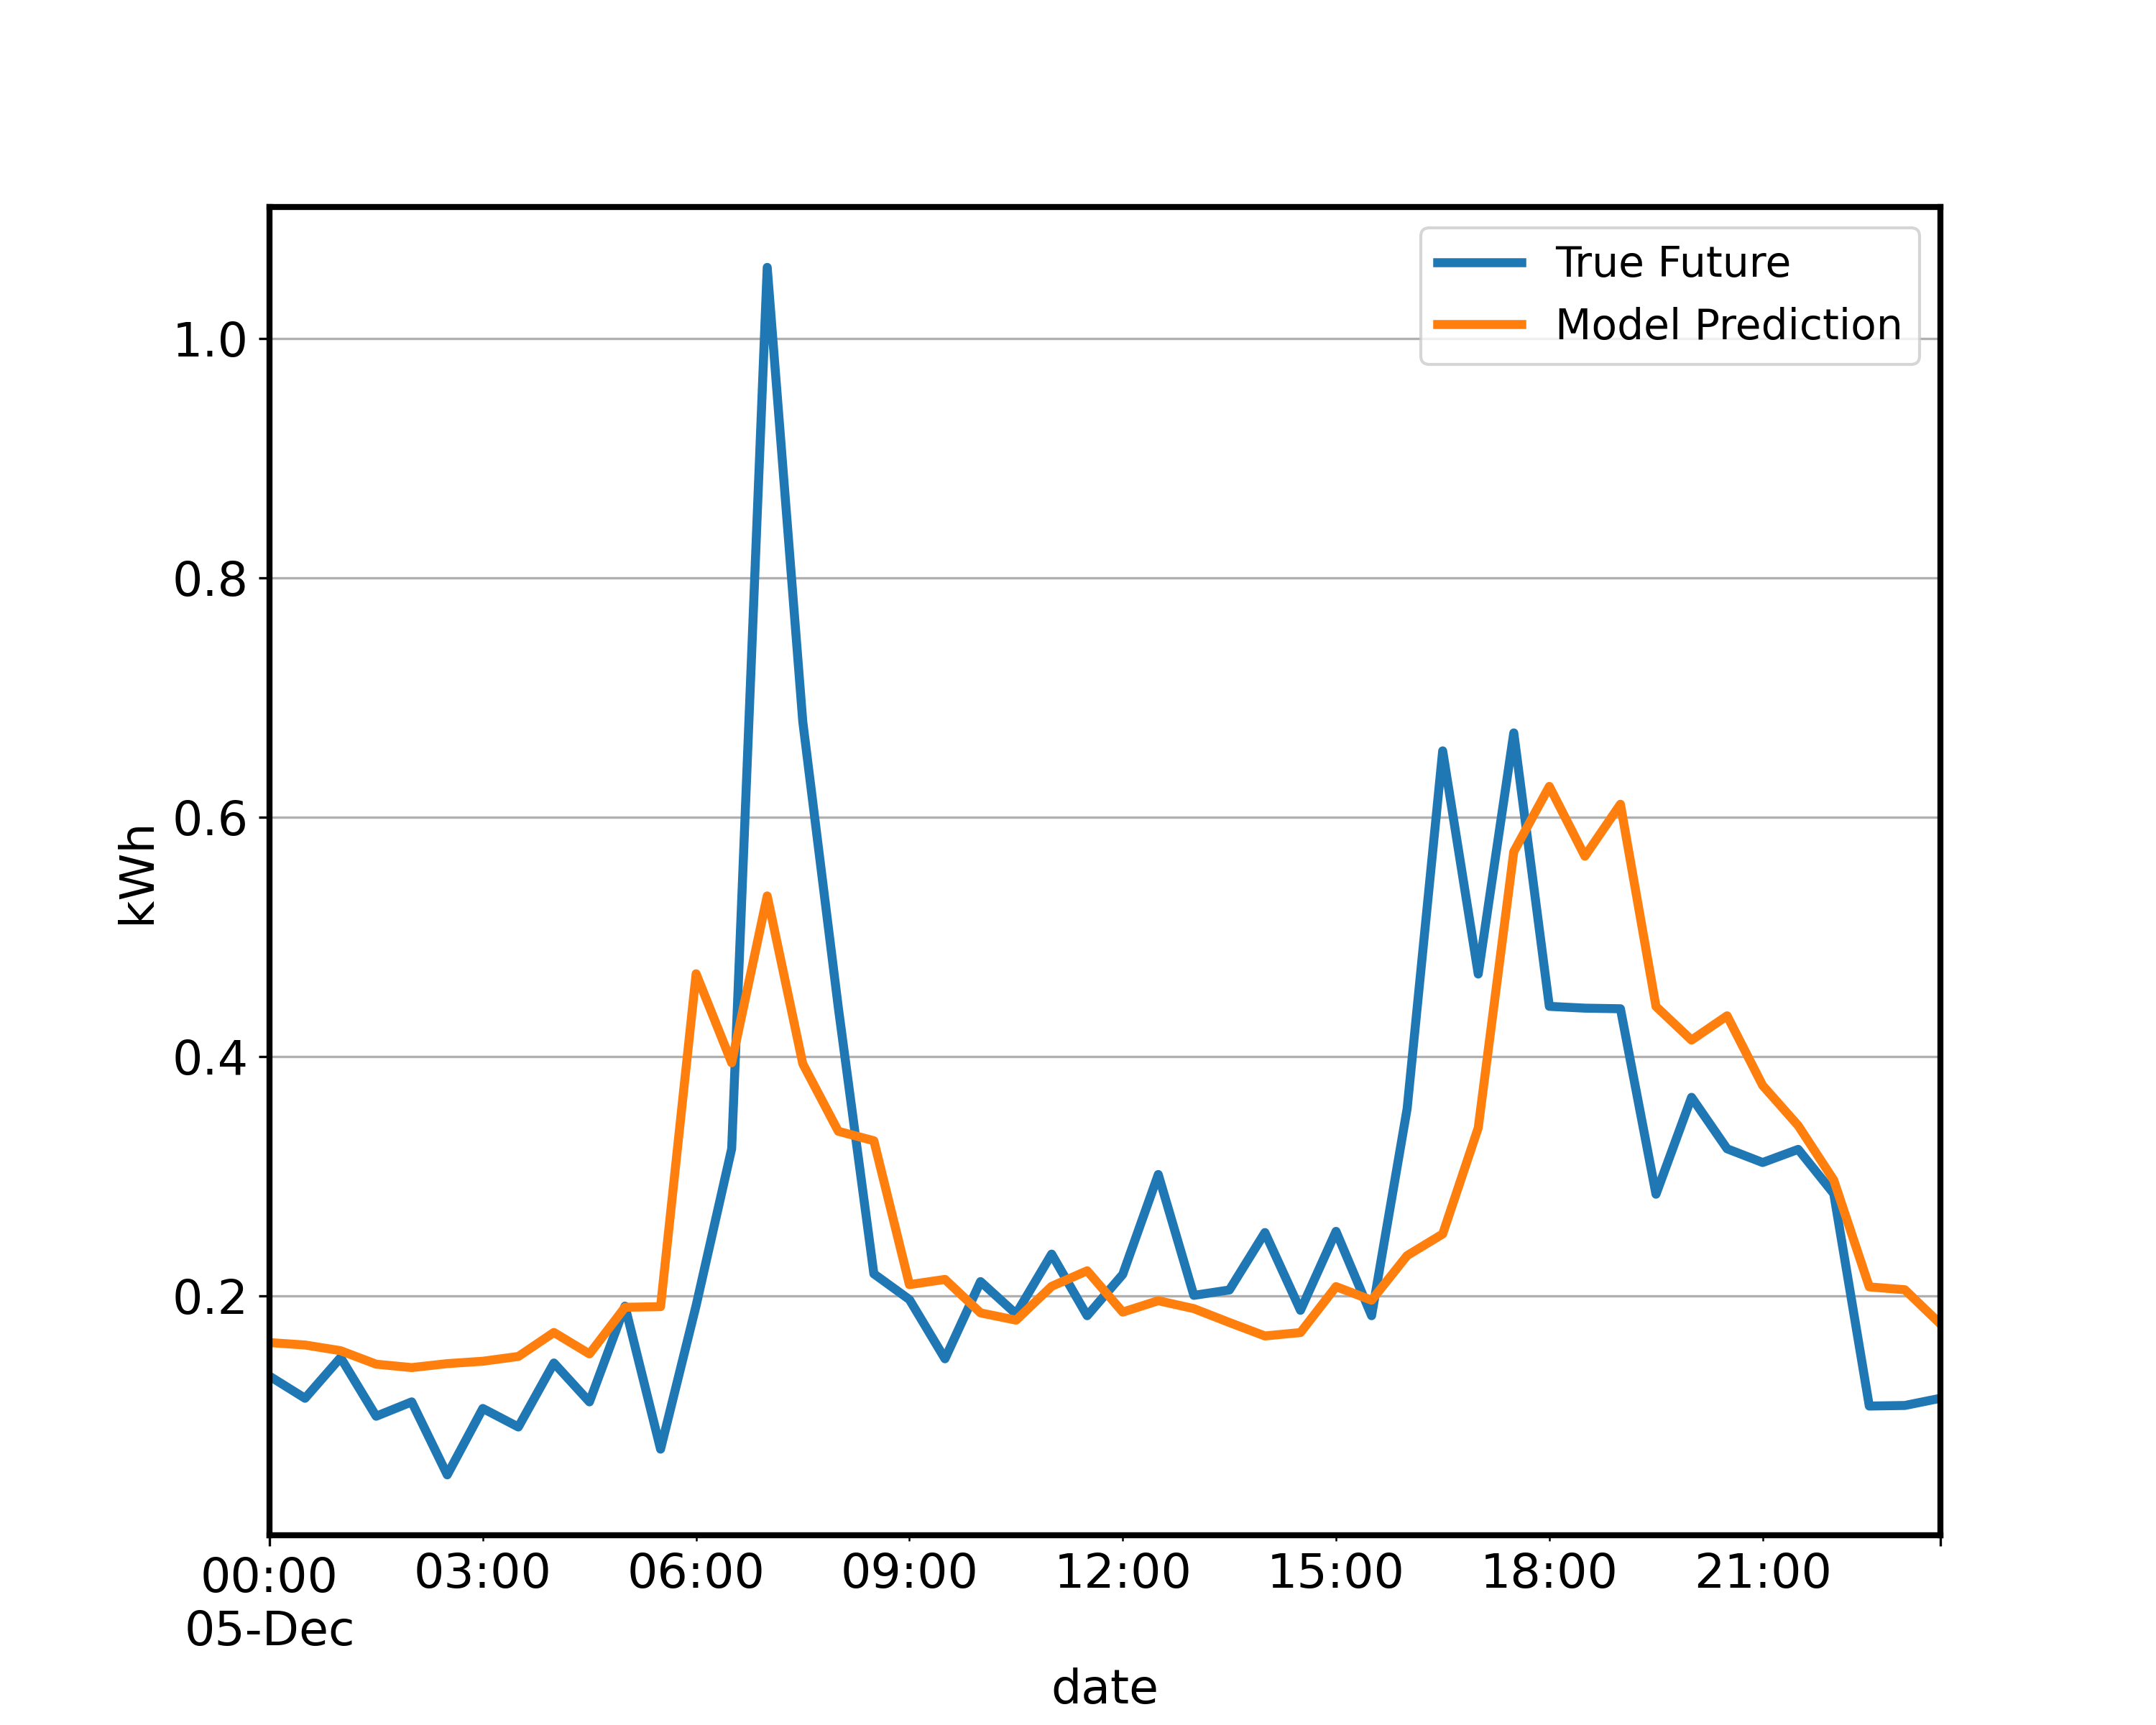
\includegraphics[width=1\linewidth]{mean_ID0x78a812ecd87a4b945e0d262aec41e0eb2b59fe1e_Day339_pred.png_1618425095.png}
		\caption{Model 4: ``Mean forecast''}
	\end{subfigure}	
	\begin{subfigure}{0.5\textwidth}
		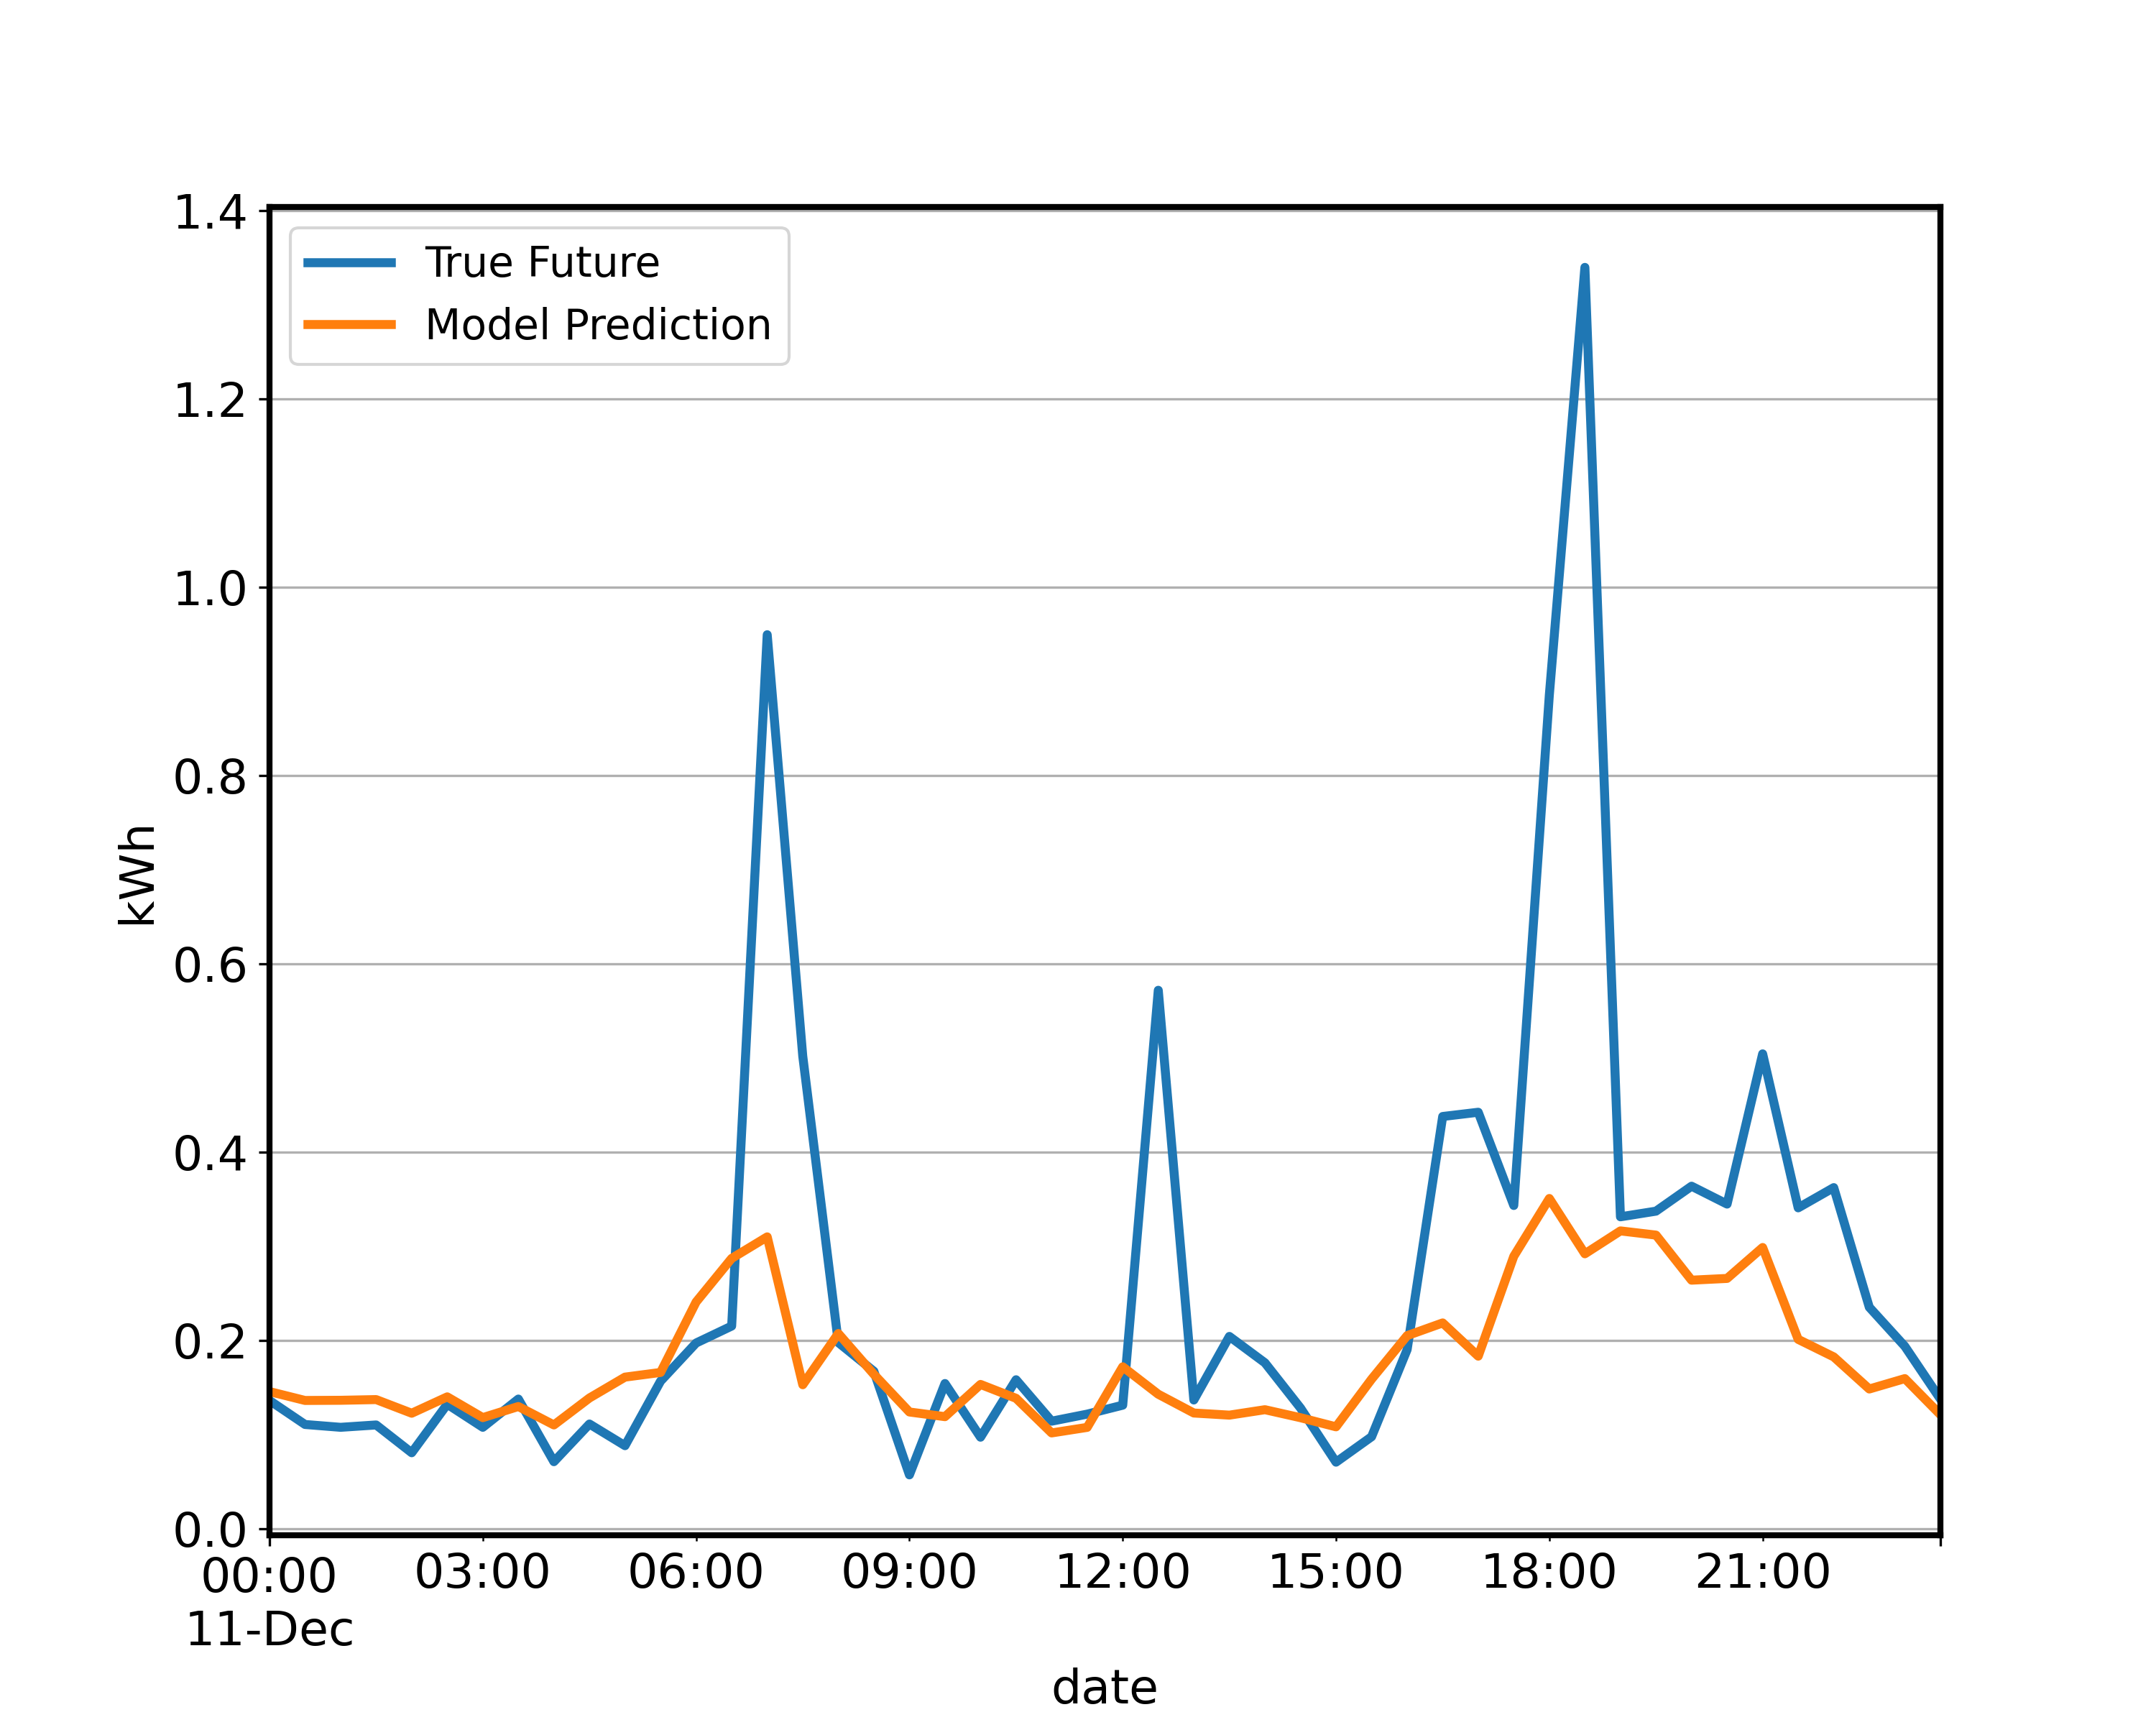
\includegraphics[width=1\linewidth]{MAPE_ID0x78a812ecd87a4b945e0d262aec41e0eb2b59fe1e_Day345_pred.png_1618425124.png}
		\caption{Model 5: ``MAPE forecast''}
	\end{subfigure}
	\caption{Daily predictions of two baseline models. (Blue: True / Orange: Prediction) }
	\label{fig:baseline models 4 and 5}
\end{figure}


Table \ref{tab:summ_data_rel_performance} shows the average performance of the baseline models on all $ 261 $ time series in the ``consumption.csv'' of Table \ref{tab:available_data} that contain a full year of measurements. The MAPE metric is not used because $ 99 $ series contain a true half hour consumption of zero, which would lead to a division by zero. The resulting error metric of every time serie is divided by the error of the model that performs worst. Then the average is taken over all the time series. The closer the averaged value is to one, the more often this model was behaving worst. By applying this normalization, the NRMSE leads to the same result as for RMSE. Therefore, only RMSE is mentioned. 

\begin{table}[ht]
	\centering
	\begin{tabular}{@{}l|ccccr@{}} \toprule
		\textbf{Error metric}	& \textbf{Closest day} & \textbf{$ 1 $ day} & \textbf{$ 7 $ days} & \textbf{mean} & \textbf{MAPE}\\\midrule
		Mean absolute error& $0.950 $&$ 0.8298 $  & $0.8224 $ & $ 0.7274 $ & $ 0.7918 $\\
		Mean squared error& $0.8377 $&$ 0.7771 $  & $0.7363 $ & $ 0.4996 $ & $ 0.6907 $\\
		Root mean square error& $0.9084 $&$ 0.8621$  & $0.8426$ & $ 0.6993$ & $ 0.8155$\\\bottomrule
	\end{tabular}
	\caption{Relative performance over all the $ 261 $ time series.}
	\label{tab:summ_data_rel_performance}
\end{table}

From Table \ref{tab:summ_data_rel_performance} it can again be concluded that the model performing a mean forecast attains the best results. The second best general applicable model over all the three metrics is the MAPE forecast model.


\section{Neural network models}\label{s:Neural network models}
\textbf{add initialization in intro!}
In this section deep LSTM and GRU models, which are models that are specialized in time series learning, are presented in different variations. The term deep is used because multiple LSTM or GRU layers are stacked on top of each other. The goal of the developed models is to make a $ 24 $ hour electrical consumption forecast of a single household. First the general context in which the deep LSTM and GRU models are trained is explained. This covers the inputs that are feeded to the models, measures taken to avoid overfitting, the explaination of a stateless model versus a stateful model and the metrics used for evaluation. Next, the specific LSTM and GRU models developed are discussed in respectively Section \ref{s:LSTM_implementation} and \ref{s:GRU_implementation}. Further, follows  the discussion of the conducted hyperparameter search in Section \ref{s:Parameter search}. Finally, the results are given and a comparison is made in Section \ref{s:Results and evaluation}.

\subsection{Different practical considerations of the models in Keras}

\subsubsection{Inputs}
The inputs to theses models are similar as was suggested in papers \cite{loadforecastingmoor} and \cite{Kong2019}: 
\begin{itemize}
	\item historic training values (min-max normalization)
	\item average daily temperature (min-max normalization)
	\item which day of the week? (one hot encoding)
	\item which time of the day? (one hot encoding)
	\item is it a holiday? (one hot encoding)
\end{itemize}

How far there will be looked back into the history of the electrical consumption is decided by the lag value. This value corresponds to the number of historic time steps that will be taken into account. The LSTM and GRU models are developed using the Keras toolbox backed by Tensorflow in Python. The Keras model expects an matrix $ X $ as input with three dimensions: sample number, amount of timesteps, amount of features. The amount of timesteps equals the lag value.

When we look at one sample of the $ X $ matrix e.g. $ (1,lag\hspace{1.5mm}value, features) $, we get a 2D matix. Timesteps corresponds to the rows of this matrix and features to the columns. Every column contains a different time serie that serves as input. On the first column an amount of $ lag\hspace{1.5mm}value $ of previous consumption values is stored. The further down the rows of the first column, the closer time gets to the actual value that needs to be predicted. This is also the case for the temperature, but because the temperature is only known on daily basis and history of the electricity consumption is known for every 30 minutes, the temperature value is often the same in the second column of the 2D matrix. The historic consumption and daily average temperature input are normalized by scaling between $ 0 $ and $ 1 $, using a min-max normalization.

In the next $ 7 $ columns of the 2D matrix, information is given about which day of the week it is. This is encoded making use of an one hot encoding.For every row one of the $ 7 $ columns which corresponds with the day of the week gets an one and the rest will be set to zero. Very similar the information about the time of the day is indicated. There are $ 48 $ columns and for every row only one column gets a one to indicate the time of the day. This makes that the 2D matrix has $ 59  $ columns which corresponds to the amount of features. Every 2D matrix in $ X $ serves as input to forecast a single next half hour electrical consumption.\\

When the 24 hour prediction is made, the assumption is taken that information about the real electrical consumption is known until the moment of prediction. In case of this thesis, that means until midnight the previous day. Because the model predicts only $ 48 $ times $ 30 $ minutes into the future, previous predictions are taken as inputs for the next.\\

\subsubsection{Stateless versus Stateful}
% $ X $ as input with three dimensions: sample number, amount of timesteps, amount of features.
Keras introduces a concept of stateless and stateful. As explained above the input given to a LSTM/GRU model is an array of data of three dimensions: sample number, amount of timesteps, amount of features. As explained in \cite{FneishMo} a stateless model interprets every row of $ X $, which is a 2D matrix of inputs, to contain in every column a serie that has nothing to do with the serie on the same column in a other sample of $ X $. When processing the next sample of $ X $, the hidden states and memory states are therefore again initialized to zero vectors. Because there is no relation between the input series over the different samples, it is logical to collect as much as possible samples for training and the input data is generated by moving a window every time one step down as can be seen in Figure \ref{fig:stateless_input}. It was further tested, that when prediction were done also the hidden states and memory states are reset for every prediction.\\

In contrast with a stateless model, a stateful model doesn't reset its hidden states and memory states when going to the next sample in $ X $. This means that when all the series that are contained in the seperate 2D matrices are sticked behind each other, the initial input signals should be recovered. How this is done can be seen in Figure \ref{fig:stateful_input} for a \textit{lag value} of three. It can however be desired to reset hidden states and memory states during training e.g. after one epoch. To achieve this, it has to be set manually. During predictions, also the hidden states and memory states are preserved. 

Using a stateful model introduces the additional complexity that the amount of training samples in $ X_{training} $ and $ X_{validation} $ should be dividable by the batch size that is chosen. A batch size is the amount of samples of $ X $ that are taken together in a batch. Additionally, this batch size also has to be used during prediction. The first problem is solved by removing samples of $ X $ at the beginning and the second issue can be workaround by transferring the trained weights to a new model with a different chosen batch size. This new model is then used during prediction.\\

Also a batch size has to be specified in the Keras fit function. For a stateful model this is equal to the earlier chosen batch size for the training model. This batchsize determines how many outputs are compared with their reference to define an objective function that is used when calculating the gradients for weight update during backpropagation through time. Because here only one sample is predicted per 2D input matrix, the amount of samples of $ X $ correspond to the amount of outputs.\\

\begin{figure}[h]
	\centering
	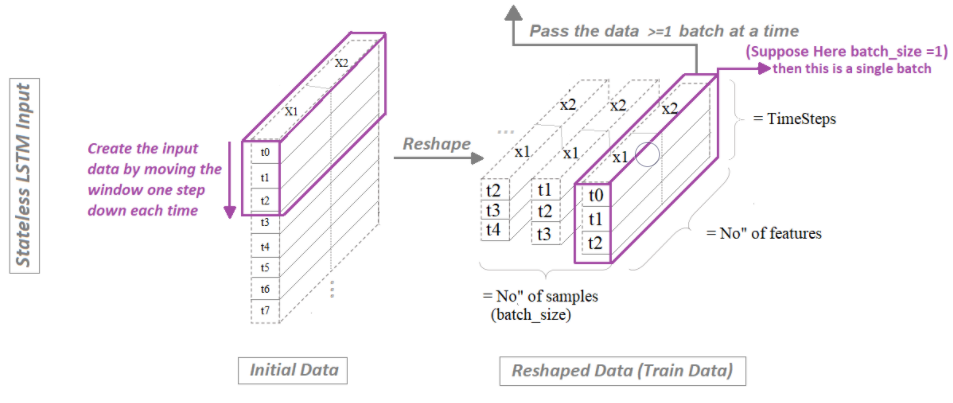
\includegraphics[width=1.2\textwidth]{stateless_input.png}
	\caption{The generation of inputs for a stateless model. (source: \cite{FneishMo})}
	\label{fig:stateless_input}
\end{figure}

\begin{figure}[h]
	\centering
	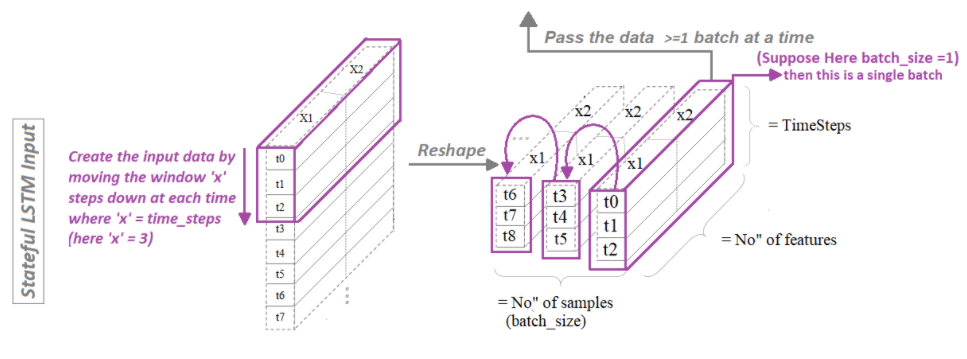
\includegraphics[width=1.2\textwidth]{stateful_input.png}
	\caption{The generation of inputs for a stateful model. (source: \cite{FneishMo})}
	\label{fig:stateful_input}
\end{figure}

\subsubsection{Initialization}
When looking at the LSTM equations in Section \ref{s:LSTM}, four weightmatrices with an index \textit{H} and four weightmatrices with a index \textit{X} can be indentified. These are respectively the recurrent and kernel weights and they are both initialized in a different way. A recurrent weight matrix is initialized using a ``orthogonal'' initialization and the kernel weight matrix uses ``glorot uniform'' initialization. Both methods are during their generation of initial values randomly sampling a distribution.\\

The biases $ \bm{b} $, memory states $ \bm{c}_t $ and hidden states $ \bm{H}_t $ of the LSTM equation are all initialized by zero arrays.\\


\subsubsection{Overfitting avoidance in Keras}
Different ways to avoid overfitting can be applied in Keras and are listed as follows:
\begin{itemize}
	\item Early Stopping
	\item Dropout and recurrent dropout in the LSTM layer
	\item Dropout in the Dense layers
	\item $ l2 $ regularization on the kernel weights, recurrent weight, bias and activity.
\end{itemize}

\subsubsection{Metrics to evaluate the models}
The metrics that are used to evaluate the prediction performance of the  neural network based models are the same as the ones used by the baseline models in Section \ref{s:Baseline models} and listed as follows:
\begin{itemize}
	\item Mean absolute error
	\item Mean squared error
	\item Normalized root mean squared error
	\item Root mean square error
	\item Mean absolute percentage error
\end{itemize}

During training also an error measure is used to accordingly update the weights of the neural network. It was found in literature that much of the time $ MSE $ is used for this.


\subsection{Deep LSTM}\label{s:LSTM_implementation}
% calculating the input data of the LSTM is done based on gpu in cloud: GPU - 1 x NVIDIA Tesla K80
% training is done on cpu with 8 threads. 
%test are done what performs fastest.
There are four different implemlentations of a deep LSTM that are being tested as listed as follows:

- make it very clear how the models work --> stateless one --> selecting a time serie from the original one --> input to LSTM --> final value is translated by a dense network. (show it graphical)

- stateless two --> same but know also take al the intermediate outputs into account for translation 

- statefull one --> sample per sample input --> takes actually only one serie into account and that is the whole serie till the day that should be predicted. The final output is then translated to a single value. (every output of the LSTM is translated to the dense network)

- statefull 48 --> each model is focussed on predicting one time moment of the day. the statefull model is shown chuncks of data. 

\begin{itemize}
	\item Stateless
	\item Stateles
\end{itemize}

%The four models I am now considering are:
%• Stateless with also last LSTM layer set to return sequence = True, whereafter a flatten layer follows--> then dense layer
%• Stateless with last LSTM return sequence = False --> then dense layer
%• A stateful model by feeding one by one the samples --> then dense layer. This means that (sample,timestep,features) has a timestep of 1.
%
%A stateful model that moves the window 48 steps down each time. Therefore, 48 models need to be build one to predict each moment of the day. This means that (sample,timestep,features) has a timestep of 48. Other multiples of 48 are also possible, but this of course decreases the number of available labels for supervised learning.


The ``long short-term memory model'' 
- model --> first lstm layers and then a dense layer.
Use of flatten layer and return sequence equal to true --> \cite{Kong2019} and add the Figure.
- use the flowchart that have sent in mail


- using cross-validation to get the accuracy of the stateless model.


\subsection{Deep GRU}\label{s:GRU_implementation}

\subsection{Parameter search}\label{s:Parameter search}
Multithreading is used to use the full potential of the CPU listed in Table \ref{tab:CPU} and simultaneously use all the available logical cores to run different threads. 

- refer back to paper LSTM: A Search Space Odyssey. There they performed a parameter search and they say that the parameters can assumed to be reasonably independent and learning rate the most important parameter. Can be learned seperately. See section \ref{s:Performance results between different models}.

- as was suggested in \cite{Greff2017}, first the learning parameter is tuned. 

- make a table of the different parameters that are varied. 

- instead of grid search --> perform a random search hyperparameter tuning.

- inspiration of the hyperparameter search comes from \cite{Shi2018}.





\subsection{Bidirectional LSTM}
In \cite{Teuwen2019} it is explain --> seems not possible, don't know the future consumptions.


\subsection{Temperature model}
A MLP model for developing a regresion model to forecast a temperature signal. 

\subsection{Results and evaluation}\ref{s:Results and evaluation}




\section{Conclusion}


%%% Local Variables: 
%%% mode: latex
%%% TeX-master: "thesis"
%%% End: 
